\chapter{Числа и свойства арифметических действий}\markright{Глава 1}
\section*{Натуральные числа: аксиомы Пеано}

Вычисления с натуральными числами опираются на небольшое число исходных положений.
Такое исходное положение называют \term{аксиомой} (axiom): в выбранной теории его принимают без доказательства,
а дальнейшие утверждения из него выводят.

\begin{definition}
\term{Натуральные числа с нулём} (natural numbers including zero) образуют множество \(\mathbb N_0\).
Для его описания выделяют начальное число \(0\) и операцию \(S\),
где \(S(n)\) означает число, следующее за \(n\).
Тройка \((\mathbb N_0,0,S)\) удовлетворяет следующим аксиомам Пеано.
\end{definition}

Запись \(n\in\mathbb N_0\) означает, что \(n\) принадлежит множеству \(\mathbb N_0\).
Буквы \(m,n\) в аксиомах обозначают произвольные его элементы.

\begin{axiom}[Начальный элемент]
\(0\in\mathbb N_0\).
\end{axiom}

\begin{axiom}[Следующее число]
Для каждого \(n\in\mathbb N_0\) определено единственное следующее число \(S(n)\in\mathbb N_0\).
\end{axiom}

\begin{axiom}[У нуля нет предшественника]
Для любого \(n\in\mathbb N_0\) выполнено \(S(n)\ne0\).
\end{axiom}

\begin{axiom}[Разные числа имеют разные следующие числа]
Если \(S(m)=S(n)\), то \(m=n\).
\end{axiom}

Последняя аксиома выражает \term{инъективность} (injectivity) операции \(S\):
равенство результатов возможно только при равенстве исходных чисел.

\begin{axiom}[Принцип математической индукции]
Пусть \(P(n)\) --- утверждение, сформулированное для \(n\in\mathbb N_0\).
Если
\begin{enumerate}[label=\arabic*.,leftmargin=2em,itemsep=3pt]
\item утверждение \(P(0)\) истинно;
\item для любого \(n\in\mathbb N_0\) из истинности \(P(n)\) следует истинность \(P(S(n))\),
\end{enumerate}
то \(P(n)\) истинно для всех \(n\in\mathbb N_0\).
\end{axiom}

\par\addvspace{5pt}\begin{lrbox}{\CatFlowBox}\begin{minipage}[t]{\linewidth}
\setlength{\parskip}{5pt}\setlength{\columnsep}{4.5mm}\setlength{\intextsep}{0pt}
\begin{wrapfigure}[13]{l}{54mm}
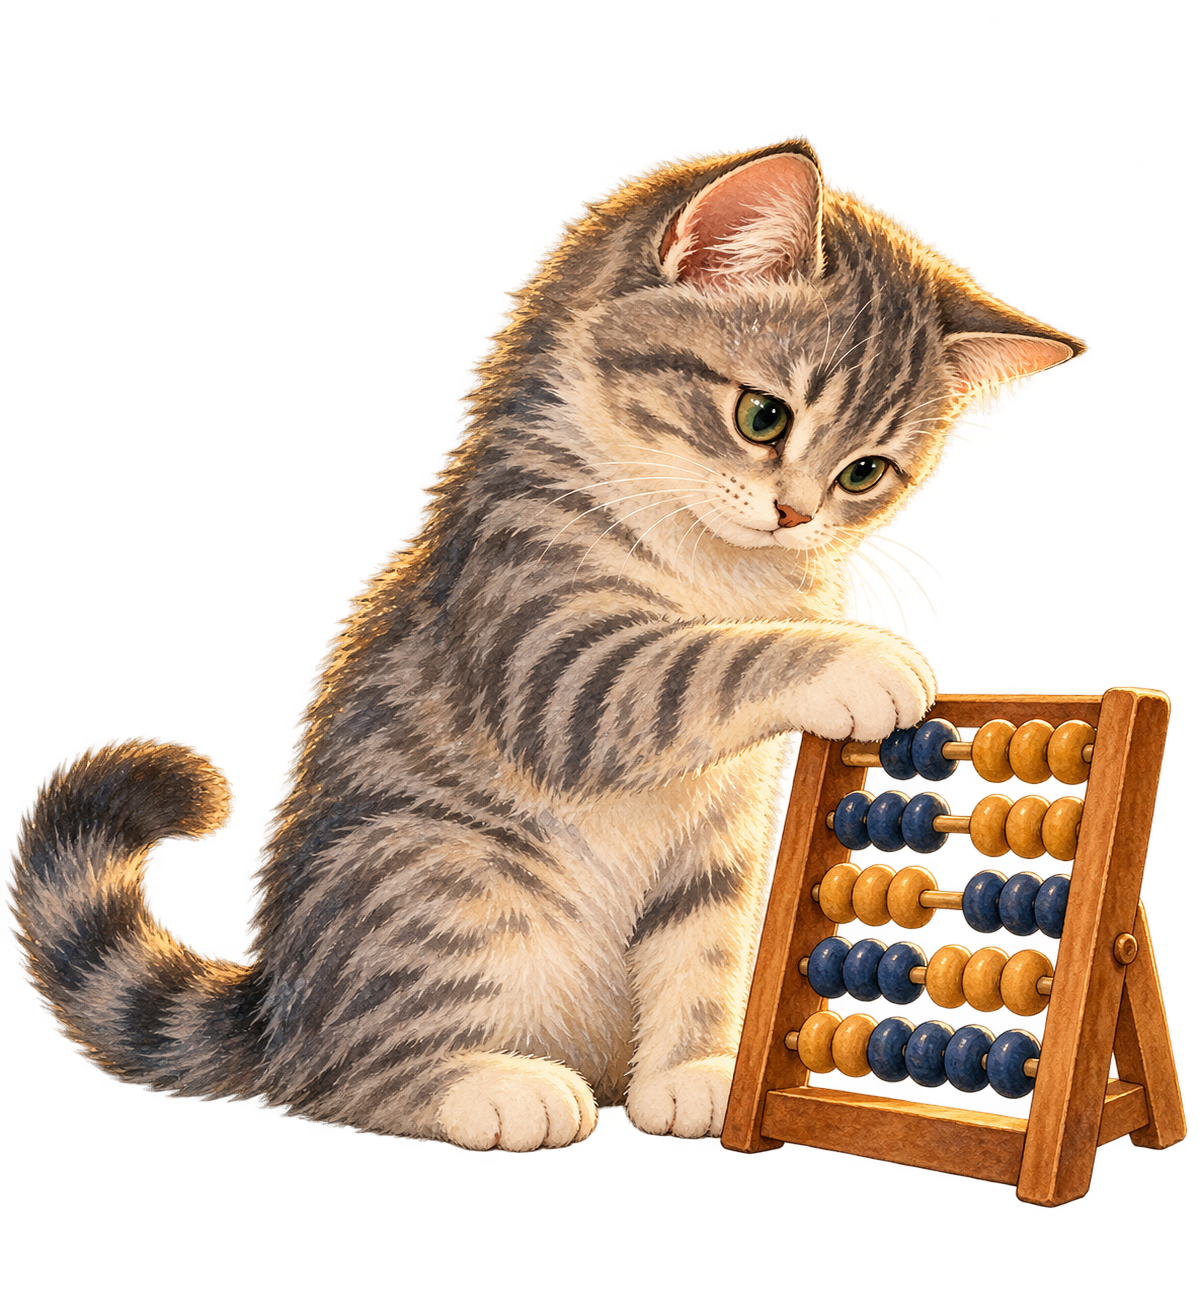
\includegraphics[width=54mm,height=58mm,keepaspectratio]{images/unique/art-02.png}
\end{wrapfigure}
В доказательстве методом \term{математической индукции} (mathematical induction)
первый пункт называют \term{базой индукции} (base case),
а второй --- \term{индукционным переходом} (inductive step).
Внутри перехода истинность \(P(n)\) временно принимают как
\term{индукционное предположение} (induction hypothesis) и из неё выводят следующий случай.
Проверка нескольких примеров не заменяет переход для произвольного \(n\).
\par\WFclear\end{minipage}\end{lrbox}%
\ifdim\dimexpr\ht\CatFlowBox+\dp\CatFlowBox\relax<64mm\dp\CatFlowBox=\dimexpr64mm-\ht\CatFlowBox\relax\fi%
\noindent\usebox{\CatFlowBox}\par\addvspace{5pt}
\begin{definition}
\term{Единица} (one) --- число \(1=S(0)\).
Далее обозначают \(2=S(1)\), \(3=S(2)\) и так далее.
\end{definition}

По аксиоме об отсутствии предшественника нуля \(1\ne0\).
Таким образом, привычная запись множества имеет вид
\[
\mathbb N_0=\{0,1,2,3,\ldots\}.
\]

\begin{definition}
\term{Натуральные числа} (natural numbers) в этом сборнике --- элементы множества
\[
\mathbb N=\mathbb N_0\setminus\{0\}=\{1,2,3,\ldots\}.
\]
Знак \(\setminus\) означает удаление указанных элементов: здесь из \(\mathbb N_0\) удалён ноль.
\end{definition}

Натуральные числа используют для счёта отдельных предметов.
Ноль соответствует отсутствию предметов, единица --- одному предмету.
В литературе встречается и соглашение \(0\in\mathbb N\), поэтому принятая здесь договорённость указана явно.

\section*{Как из следования получаются сложение и умножение}

\begin{definition}
\term{Рекурсивное определение} (recursive definition) задаёт начальное значение
и правило получения следующего значения из уже определённого.
Для \(a,b\in\mathbb N_0\) сложение и умножение задают правилами
\[
\begin{aligned}
a+0&=a, & a+S(b)&=S(a+b),\\
a\cdot0&=0, & a\cdot S(b)&=a\cdot b+a.
\end{aligned}
\]
\end{definition}

Например,
\[
a+1=a+S(0)=S(a+0)=S(a).
\]
Поэтому после введения сложения вместо \(S(n)\) можно писать \(n+1\).
В индукционном переходе тогда доказывают \(P(n+1)\), предполагая \(P(n)\).
Если утверждение сформулировано только для \(n\ge1\), базой служит случай \(n=1\).

Следующие два доказательства показывают, как привычные свойства действий выводятся из определений.

\begin{theorem}[Ноль слева при сложении]
Для любого \(n\in\mathbb N_0\) выполнено \(0+n=n\).
\end{theorem}

\begin{proof}
База: при \(n=0\) рекурсивное определение даёт \(0+0=0\).
Переход: предположим, что \(0+n=n\). Тогда
\[
0+S(n)=S(0+n)=S(n).
\]
Значит, утверждение верно и для следующего числа. По принципу индукции оно верно для всех \(n\in\mathbb N_0\).
\end{proof}

Теперь рекурсивное правило умножения даёт
\[
a\cdot1=a\cdot S(0)=a\cdot0+a=0+a=a.
\]

\begin{theorem}[Ассоциативность сложения]
Для любых \(a,b,c\in\mathbb N_0\)
\[
(a+b)+c=a+(b+c).
\]
\end{theorem}

\par\addvspace{5pt}\begin{lrbox}{\CatFlowBox}\begin{minipage}[t]{\linewidth}
\setlength{\parskip}{5pt}\setlength{\columnsep}{4.5mm}\setlength{\intextsep}{0pt}
\begin{wrapfigure}[13]{l}{54mm}

\includegraphics[width=54mm,height=58mm,keepaspectratio]{images/unique/art-04.png}
\end{wrapfigure}
\textit{Доказательство.} Зафиксируем произвольные \(a,b\in\mathbb N_0\) и проведём индукцию по \(c\).
База \(c=0\):
\[
(a+b)+0=a+b=a+(b+0).
\]
Предположим, что \((a+b)+c=a+(b+c)\). По рекурсивному правилу сложения
\[
\begin{aligned}
(a+b)+S(c)
&=S\bigl((a+b)+c\bigr)\\
&=S\bigl(a+(b+c)\bigr)\\
&=a+S(b+c)\\
&=a+\bigl(b+S(c)\bigr).
\end{aligned}
\]
Переход доказан. Принцип индукции завершает доказательство.\hfill\(\square\)
\par\WFclear\end{minipage}\end{lrbox}%
\ifdim\dimexpr\ht\CatFlowBox+\dp\CatFlowBox\relax<64mm\dp\CatFlowBox=\dimexpr64mm-\ht\CatFlowBox\relax\fi%
\noindent\usebox{\CatFlowBox}\par\addvspace{5pt}


\begin{definition}
\term{Целые числа} (\emph{integers}) --- натуральные числа, противоположные им отрицательные числа и ноль:
\[
\mathbb Z=\{\ldots,-3,-2,-1,0,1,2,3,\ldots\}.
\]
\end{definition}

\begin{definition}
\term{Противоположное число} (\emph{additive inverse}) к числу \(a\) --- число \(-a\), сумма которого с \(a\) равна нулю:
\[
a+(-a)=0.
\]
Например, \(5\) и \(-5\) противоположны; число, противоположное нулю, --- сам ноль.
\end{definition}

На числовой прямой число тем больше, чем правее находится его точка.
Например, \(-8<-3<0<4\).
Запись \(a\in\mathbb Z\) читается: «\(a\) принадлежит множеству целых чисел».

\section*{Действия с целыми числами}

Сумма, разность и произведение целых чисел всегда являются целыми числами.
Деление может вывести за пределы целых чисел: например, \(6:3=2\), но \(1:2\) не является целым числом.

Вычитание означает прибавление противоположного числа:
\[
a-b=a+(-b),\qquad a-(-b)=a+b.
\]
При сложении двух отрицательных чисел складывают их расстояния до нуля и ставят минус:
\[
(-7)+(-5)=-12.
\]
При сложении чисел разных знаков из большего расстояния до нуля вычитают меньшее
и берут знак числа, расположенного дальше от нуля:
\[
-14+9=-5,\qquad -9+14=5,\qquad -9+9=0.
\]
При умножении или делении двух ненулевых чисел одинаковые знаки дают плюс, разные --- минус:
\[
(-6)(-4)=24,\qquad (-6)\cdot4=-24,\qquad
\frac{-24}{-6}=4,\qquad \frac{24}{-6}=-4.
\]
Деление на ноль не определено; в частности, запись \(\frac{0}{0}\) также не имеет значения.

\section*{От целых чисел к рациональным}

\begin{definition}
\term{Рациональное число} (\emph{rational number}) --- число, которое можно записать в виде
\[
\frac pq,\qquad p\in\mathbb Z,\quad q\in\mathbb Z,\quad q\ne0.
\]
Множество рациональных чисел обозначают \(\mathbb Q\).
\end{definition}

Любое целое число рационально, поскольку \(n=\frac n1\).
Например, \(3\), \(-2\), \(0\), \(\frac12\) и \(-\frac34\) --- рациональные числа.
Правила действий с дробями подробно разобраны в главе 3.
Следующие свойства удобно сформулировать сразу для всех рациональных чисел:
ими пользуются и при вычислениях, и при дальнейших преобразованиях выражений с буквами.

\section*{Основные свойства арифметических действий}

Во всех формулах ниже \(a,b,c\) --- произвольные рациональные числа.

\textbf{Замкнутость сложения и умножения.}
Сумма и произведение рациональных чисел снова рациональны:
\[
a+b\in\mathbb Q,\qquad ab\in\mathbb Q.
\]
Разность также рациональна; частное рационально при ненулевом делителе.

\par\addvspace{5pt}\begin{lrbox}{\CatFlowBox}\begin{minipage}[t]{\linewidth}
\setlength{\parskip}{5pt}\setlength{\columnsep}{4.5mm}\setlength{\intextsep}{0pt}
\begin{wrapfigure}[9]{r}{54mm}

\includegraphics[width=54mm,height=58mm,keepaspectratio]{images/unique/art-03.png}
\end{wrapfigure}
\textbf{Коммутативность} (переместительный закон).
Перестановка слагаемых или множителей не меняет результата:
\[
a+b=b+a,\qquad ab=ba.
\]

\textbf{Ассоциативность} (сочетательный закон).
Группировка слагаемых или множителей не меняет результата:
\[
(a+b)+c=a+(b+c),\qquad (ab)c=a(bc).
\]

\textbf{Нейтральные элементы.}
Прибавление нуля и умножение на единицу не меняют число:
\[
a+0=0+a=a,\qquad a\cdot1=1\cdot a=a.
\]
Поэтому \(0\) называют нейтральным элементом сложения,
а \(1\) --- нейтральным элементом умножения.
\par\WFclear\end{minipage}\end{lrbox}%
\ifdim\dimexpr\ht\CatFlowBox+\dp\CatFlowBox\relax<64mm\dp\CatFlowBox=\dimexpr64mm-\ht\CatFlowBox\relax\fi%
\noindent\usebox{\CatFlowBox}\par\addvspace{5pt}
\textbf{Противоположное число.}
У каждого числа есть противоположное:
\[
a+(-a)=(-a)+a=0.
\]

\begin{definition}
\term{Обратное число} (\emph{multiplicative inverse; reciprocal}) к ненулевому числу \(a\) --- число \(\frac1a\),
произведение которого с \(a\) равно единице:
\[
a\cdot\frac1a=\frac1a\cdot a=1,\qquad a\ne0.
\]
\end{definition}
Например, \(2\) и \(\frac12\) взаимно обратны.
У нуля обратного числа нет. Деление заменяется умножением на обратное число:
\[
\frac ab=a\cdot\frac1b,\qquad b\ne0.
\]

\textbf{Дистрибутивность} (распределительный закон).
Умножение распределяется относительно сложения:
\[
a(b+c)=ab+ac,\qquad (a+b)c=ac+bc.
\]
Для разности соответственно \(a(b-c)=ab-ac\).

\textbf{Умножение на ноль и правила знаков.}
Из перечисленных свойств следуют равенства
\[
a\cdot0=0,\qquad (-a)b=-(ab),\qquad (-a)(-b)=ab.
\]

\textbf{Законы сокращения.}
Прибавление одного числа к обеим частям равенства можно отменить;
умножение можно отменить, если общий множитель ненулевой:
\[
a+c=b+c\ \Longrightarrow\ a=b,
\]
\[
ac=bc,\quad c\ne0\ \Longrightarrow\ a=b.
\]
Знак \(\Longrightarrow\) означает «из этого следует».

\textbf{Свойство нулевого произведения.}
Произведение равно нулю тогда и только тогда, когда хотя бы один множитель равен нулю:
\[
ab=0\quad\Longleftrightarrow\quad a=0\ \text{или}\ b=0.
\]
Знак \(\Longleftrightarrow\) означает, что утверждения равносильны: каждое следует из другого.

Коммутативность и ассоциативность относятся к сложению и умножению.
Переносить их на вычитание и деление нельзя:
\[
7-2\ne2-7,\qquad (12:3):2\ne12:(3:2).
\]

\section*{Порядок действий}

\begin{enumerate}[label=\arabic*.,leftmargin=2em,itemsep=3pt]
\item Действия в скобках, начиная с самых внутренних.
\item Возведение в степень. Например, \(3^2=3\cdot3\).
\item Умножение и деление --- слева направо.
\item Сложение и вычитание --- слева направо.
\end{enumerate}

Степень относится только к своему основанию:
\[
(-3)^2=9,\qquad -3^2=-(3^2)=-9.
\]
Например,
\[
-3-(-5)\cdot2=-3-(-10)=-3+10=7.
\]

\section*{Порядок на числовой прямой}
Для любых рациональных \(a,b\) выполняется ровно одно из условий: \(a<b\), \(a=b\), \(a>b\).
Если \(a<b\) и \(b<c\), то \(a<c\) — это \textbf{транзитивность}.
Из \(a<b\) следует \(a+c<b+c\). Если также \(c>0\), то \(ac<bc\); если \(c<0\), то \(ac>bc\).
Эти правила объясняют преобразования неравенств в главе 11.
\Needspace{7\baselineskip}\section*{Задачи}
\begingroup\setlength{\parskip}{3pt}
\noindent\begin{minipage}[t]{\linewidth}\textbf{1.1.} Сравни: \(- 8\) и \(- 3;\allowbreak 0\) и \(- 5;\allowbreak - 4\) и \(4\).\par\end{minipage}\par
\noindent\begin{minipage}[t]{\linewidth}\textbf{1.2.} Вычисли: \(- 7 + (- 5)\).\par\end{minipage}\par
\noindent\begin{minipage}[t]{\linewidth}\textbf{1.3.} Вычисли: \(- 14 + 9 + 8\).\par\end{minipage}\par
\noindent\begin{minipage}[t]{\linewidth}\textbf{1.4.} Вычисли: \(6 - (- 4) - 13\).\par\end{minipage}\par
\noindent\begin{minipage}[t]{\linewidth}\textbf{1.5.} Вычисли: \((- 6) \cdot  (- 4) : (- 3)\).\par\end{minipage}\par
\noindent\begin{minipage}[t]{\linewidth}\textbf{1.6.} Вычисли: \(0 \cdot  (- 15) + 0 : (- 3) + 7\). Можно ли вычислить \(7 : 0\)?\par\end{minipage}\par
\noindent\begin{minipage}[t]{\linewidth}\textbf{1.7.} Вычисли: \(18 - 4 \cdot  7 + 12 : (- 3)\).\par\end{minipage}\par
\noindent\begin{minipage}[t]{\linewidth}\textbf{1.8.} Вычисли: \(48 : (- 6) \cdot  2 - 9 + 5\).\par\end{minipage}\par
\par\addvspace{5pt}\begin{lrbox}{\CatFlowBox}\begin{minipage}[t]{\linewidth}
\setlength{\parskip}{5pt}\setlength{\columnsep}{4.5mm}\setlength{\intextsep}{0pt}
\begin{wrapfigure}[9]{r}{54mm}

\includegraphics[width=54mm,height=58mm,keepaspectratio]{images/unique/art-05.png}
\end{wrapfigure}
\textbf{1.9.} Вычисли: \(- 3 \cdot  [8 - (5 - 9)] + 10\).\par

\textbf{1.10.} Вычисли: \((- 3)^{2} - 3^{2} + (- 2)^{3} - (- 2^{2})\).\par

\textbf{1.11.} Из жизни. Утром было \(- 6 {}^{\circ} C\). К полудню потеплело на \(9 {}^{\circ} C\), а вечером похолодало на \(5 {}^{\circ} C\). Какая температура стала вечером?\par

\textbf{1.12.} Из жизни. Лифт находился на уровне \(- 2\) подземной парковки, поднялся на \(7\) уровней и опустился на \(3\). На каком уровне он оказался? Уровень земли обозначен \(0\), уровни идут подряд.\par

\textbf{1.13.} Из жизни. На игровом счёте было \(120\) очков. За каждую из трёх ошибок сняли \(15\) очков, затем начислили \(40\) очков. Сколько очков осталось?\par

\textbf{1.14.}\starmark{} Вычисли: \(- 48 : [6 - 2 \cdot  (- 1)] + 3 \cdot  [- 4 - (- 7)]\).\par

\textbf{1.15.}\starmark{} Подставь скобки в \(18 - 6 : 3 + 1\), сохранив порядок чисел и действий, чтобы получилось \(3\).\par
\par\WFclear\end{minipage}\end{lrbox}%
\ifdim\dimexpr\ht\CatFlowBox+\dp\CatFlowBox\relax<64mm\dp\CatFlowBox=\dimexpr64mm-\ht\CatFlowBox\relax\fi%
\noindent\usebox{\CatFlowBox}\par\addvspace{5pt}

\noindent\begin{minipage}[t]{\linewidth}\textbf{1.16.}\starmark{} В викторине за верный ответ дают \(5\) очков, за неверный снимают \(3\). Участник ответил на все \(12\) вопросов и набрал \(28\) очков. Сколько было верных ответов?\par\end{minipage}\par
\noindent\begin{minipage}[t]{\linewidth}\textbf{1.17.} Докажи математической индукцией, что \(\sum_{k=1}^{n}k=\dfrac{n(n+1)}2\) для всех \(n\in\mathbb N_0\). Знак \(\sum\) обозначает сумму слагаемых при указанных значениях индекса; при \(n=0\) сумма пуста и равна \(0\).\par\end{minipage}\par
\noindent\begin{minipage}[t]{\linewidth}\textbf{1.18.} Докажи математической индукцией: \(1+3+\cdots+(2n-1)=n^2\) для всех \(n\in\mathbb N\).\par\end{minipage}\par
\noindent\begin{minipage}[t]{\linewidth}\textbf{1.19.}\starmark{} Докажи математической индукцией: \(\sum_{k=1}^{n}k^2=\dfrac{n(n+1)(2n+1)}6\) для всех \(n\in\mathbb N_0\). Пустая сумма равна нулю.\par\end{minipage}\par
\noindent\begin{minipage}[t]{\linewidth}\textbf{1.20.} Докажи математической индукцией: \(\sum_{k=0}^{n}2^k=2^{n+1}-1\) для всех \(n\in\mathbb N_0\). Здесь \(2^0=1\).\par\end{minipage}\par
\noindent\begin{minipage}[t]{\linewidth}\textbf{1.21.} Докажи математической индукцией: \(3^n\ge2n+1\) для всех \(n\in\mathbb N_0\). Здесь \(3^0=1\).\par\end{minipage}\par
\noindent\begin{minipage}[t]{\linewidth}\textbf{1.22.} Докажи математической индукцией: \(2^n\ge n^2\) для всех целых \(n\ge4\).\par\end{minipage}\par
\noindent\begin{minipage}[t]{\linewidth}\textbf{1.23.}\starmark{} Докажи математической индукцией: \(\sum_{k=1}^{n}k^3=\left(\dfrac{n(n+1)}2\right)^2\) для всех \(n\in\mathbb N_0\). Пустая сумма равна нулю.\par\end{minipage}\par
\noindent\begin{minipage}[t]{\linewidth}\textbf{1.24.}\starmark{} Докажи индукцией по натуральному \(n\) неравенство Бернулли: \((1+x)^n\ge1+nx\) для любого рационального \(x\ge-1\). Объясни, почему условие \(1+x\ge0\) нужно в индукционном переходе.\par\end{minipage}\par
\noindent\begin{minipage}[t]{\linewidth}\textbf{1.25.} Докажи единственность противоположного рационального числа: если \(a+x=0\) и \(a+y=0\), то \(x=y\). Используй свойства сложения.\par\end{minipage}\par
\noindent\begin{minipage}[t]{\linewidth}\textbf{1.26.} Докажи свойство нулевого произведения для рациональных чисел: \(ab=0\) тогда и только тогда, когда \(a=0\) или \(b=0\).\par\end{minipage}\par
\endgroup
